
\section{Introduction}\label{sec:intro}
If things are free (or even cheap), spam arrives. The “free” CA needs to cost
at least something. The proposals below are to place some cost on each request
when money is not being spent. In other words: requests must be paid for with
the requestor’s time.

\begin{multicols}{2}

Very few clients like the idea of leaving a checkbook open during construction
so it's not uncommen for construction administration to be structured as a
fixed fee for a contract.

But no matter how much work goes into exclusions and protections in the
language of the contract to clarify the limitation of the services, the hiring
party ends up frustrated with ever having to pay more soft costs once the
construction starts.

And so how can a constractural relationship be in place that ensures the client
is not innundated with soft cost changes orders while continuing to receive a
reasonable level of service from the professional?

One of the common problems lies in the fact that engineers are only called on
during construction when there is a problem. This often creates a
guilty-until-proven innocent scenario for the engineer. The engineer feels
obliged to look into the issue and more often than not concludes, after hours
of research, that the problem was not the design. But who pays for that?

Now that the engineer is cleared from a claim that was being threatened, they
will certainly be asked immediately afterward if they can update the drawings
and help find a solution. In this scenario, not only are they not offered
compensation for the trial they were just on but now are expected to perform
some level of engineering for free.

This all compounds in on itself because doing the work without charging means
the engineer accepts all of the risk with no reward. They are often rushed to
solve a problem they did not create, and if they make an error they will be
held legally responsible. This can range anywhere from economic damage to their
reputation, to a claim to pay for the error, to a loss of license depending on
the severity of this error.

Their only other option is to say no to the request. But this will be at the
economic cost of not being a team player.

The engineer might ask for a change order, but that is always politically
challenging since the professional service doesn't buy a "thing" and so it only
creates tension and anger between parties.

Ultimately the engineer is put in a situation where they must decide between
damaging their financial wellbeing by trying to charge or damaging their
financial wellbeing by obliging the request and completing the task for free.

So why is it that we accept this practice? Putting a professional in a
situation

This is the first line of the report. This report will document things.

This test. the text will wrap around properly don't you worry okay there so
here we go!!

Example citation. \cite{kenny, ricardo}



\begin{figure}[H]
    \centering
    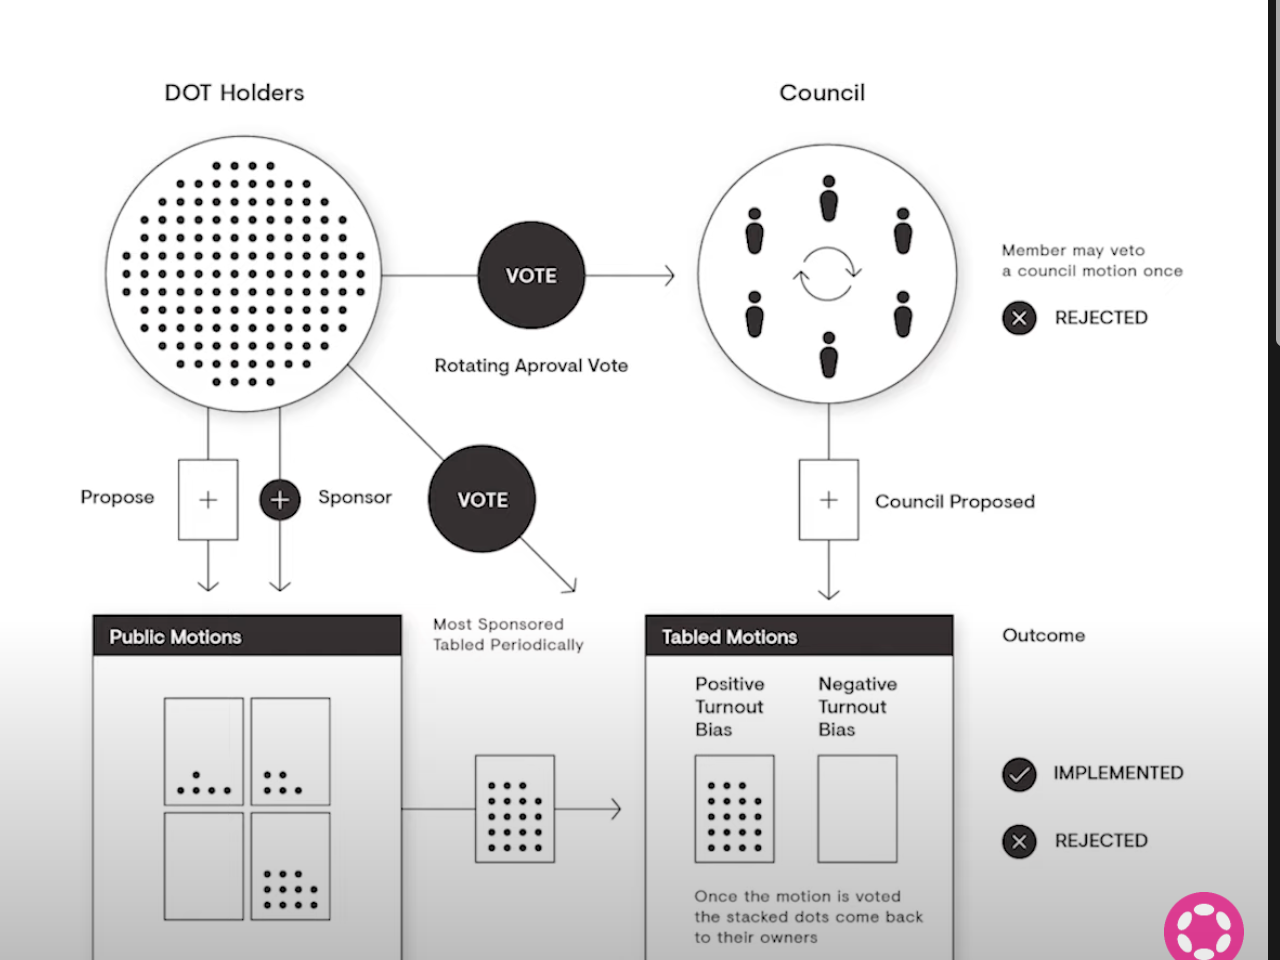
\includegraphics[height=1in]{./document/img/example.png}
    \caption[Optional caption]{Real, local caption}
    \label{fig:example}
\end{figure}

Figure \ref{fig:example} shows an example.